\begin{frame}{A brief introduction}
   ``Machine learning, neural networks, and artificial intelligence are increasingly being used in orthopaedics for image processing and analysis tasks. These techniques can be used to {\bf automatically analyze medical images} such as X-rays, MRI scans, and CT scans to {\bf extract important diagnostic information} and help with diagnosis and treatment planning. Machine learning algorithms can be trained to {\bf recognize patterns in the images}, and neural networks can be used to process and interpret the data in a more human-like way. These approaches can be used to {\bf identify abnormalities, measure bone density, and classify different types of tissue}, among other tasks. By automating these processes, doctors and other healthcare professionals can {\bf save time and improve the accuracy of their diagnoses}'' \\
\vspace{5mm}
   \hfill - ChatGPT (emphasis mine)
\end{frame}

\begin{frame}{Three main types}
   \begin{fullpageitemize}
         \item \centering \largetext{Classification}
         \item \centering \largetext{Segmentation}
         \item \centering \largetext{Regression}
      \end{fullpageitemize}
\end{frame}

\framecard[colorblue]{{\color{white}\hugetext{EXAMPLES}}}

\begin{frame}
   \centering
      
\includegraphics[width=\linewidth]{images/histology-title.png}
      \vfill
      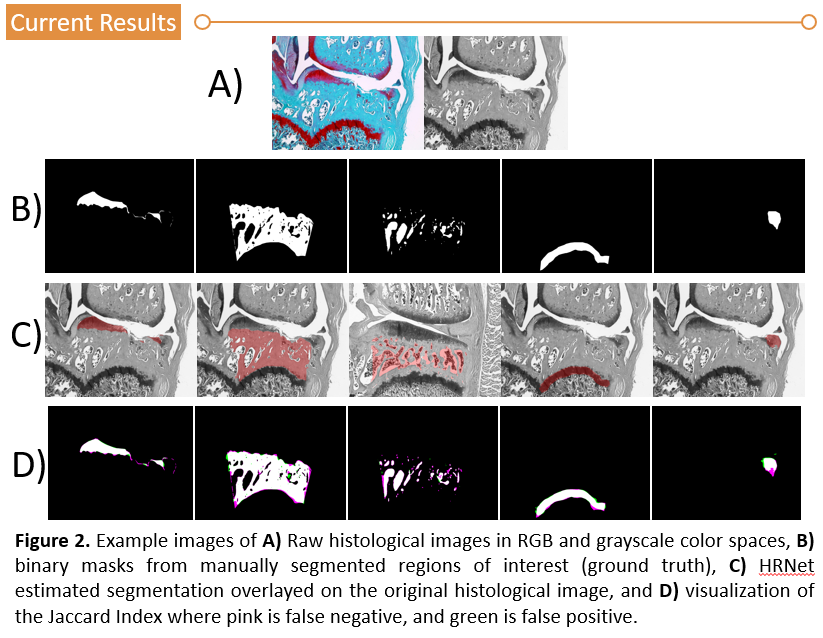
\includegraphics[width=0.65\linewidth]{images/histology-images.png}
\end{frame}

\begin{frame}
   \centering
   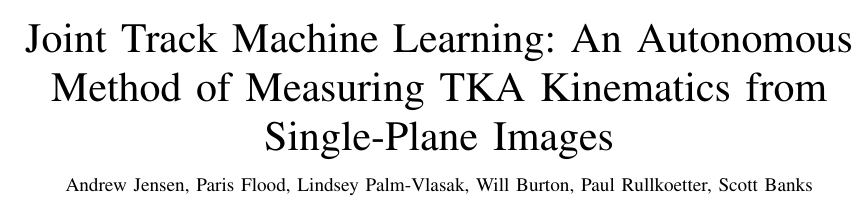
\includegraphics[width=0.78\linewidth]{images/jtml-title.png}
   \vfill
   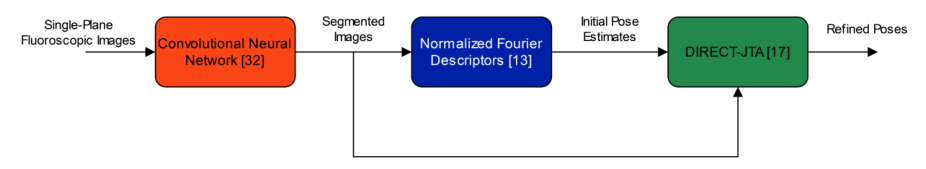
\includegraphics[width=0.75\linewidth]{images/jtml-pipeline.png}
   \vfill
   \begin{columns}
      \begin{column}{0.71\linewidth}
         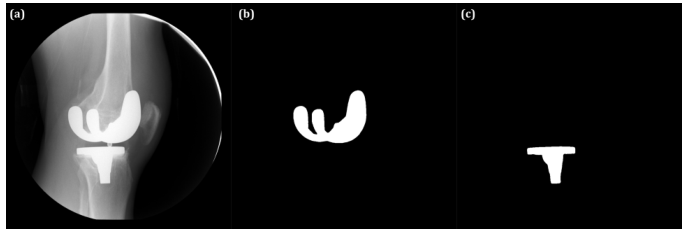
\includegraphics[width=\columnwidth]{images/jtml-nn-image.png}
      \end{column}
      \begin{column}{0.29\linewidth}
         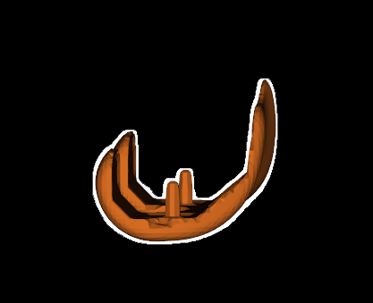
\includegraphics[width=\columnwidth]{images/jtml-registered-implant.png}
      \end{column}
   \end{columns}
\end{frame}

\begin{frame}{Classification of Equine Stifle Pathology}
   \centering
   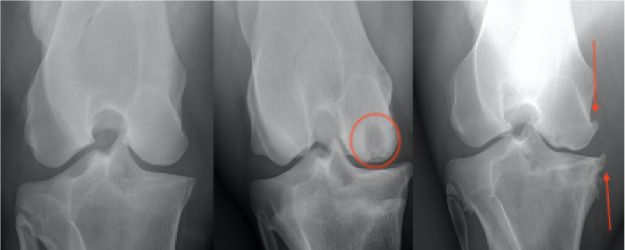
\includegraphics[width=0.85\linewidth]{images/stifle-pathologies.png}
\end{frame}

\begin{frame}
   \centering
   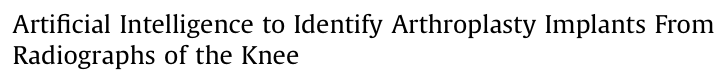
\includegraphics[width=0.7\linewidth]{images/tka-classification-title.png}
   \begin{columns}
      \begin{column}{0.6\linewidth}
         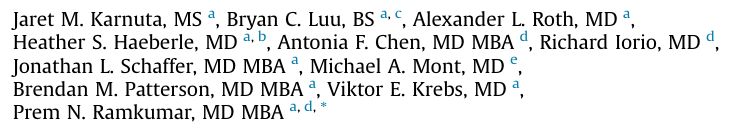
\includegraphics[width=\columnwidth]{images/tka-classification-authors.png}
      \end{column}
      \begin{column}{0.5\linewidth}
         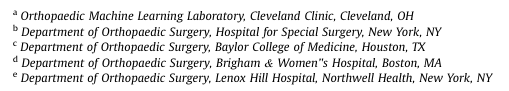
\includegraphics[width=\columnwidth]{images/tka-classification-universities.png}
      \end{column}
   \end{columns}
   \vfill
   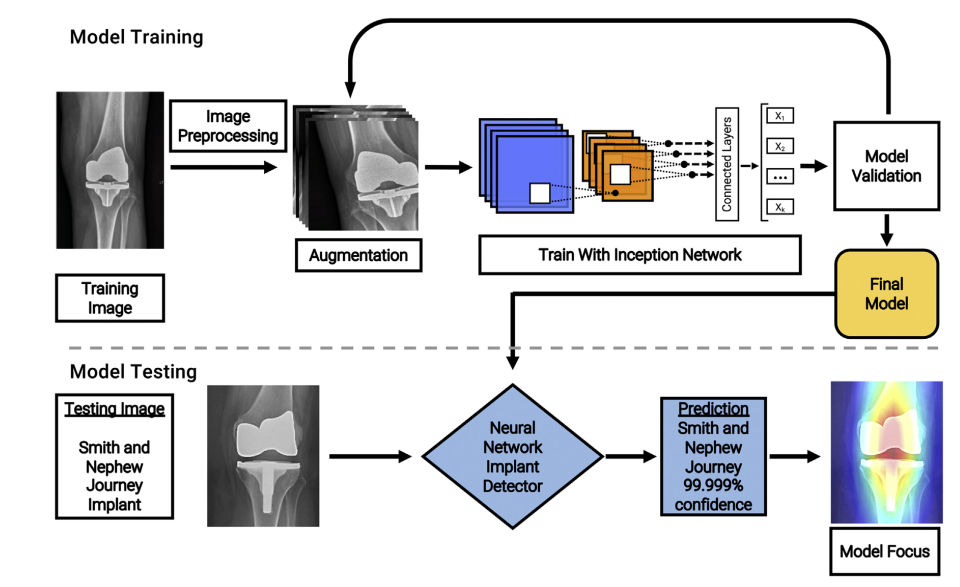
\includegraphics[width=0.65\linewidth]{images/tka-classification.png}
\end{frame}

\begin{frame}
   \centering
   \begin{columns}
      \begin{column}{0.65\linewidth}
         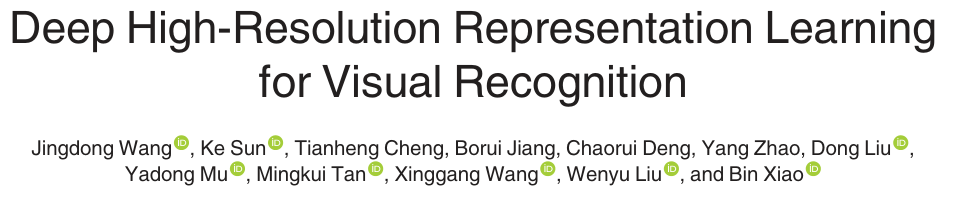
\includegraphics[width=\columnwidth]{images/hrnet-title.png}
      \end{column}
      \begin{column}{0.35\linewidth}
         
\includegraphics[width=\columnwidth]{images/hrnet-authors.png}
      \end{column}
   \end{columns}
   \vfill
   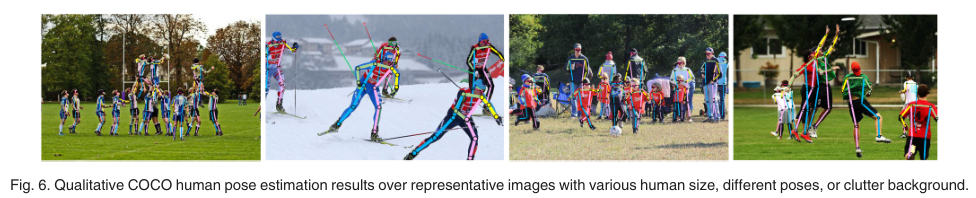
\includegraphics[width=\linewidth]{images/hrnet-human-pose.png}
\end{frame}

\begin{frame}{Open Source Fonts}
 \begin{fullpageitemize}
  \item {\montserratfont This is Montserrat}
  \item {\notosansfont This is Noto Sans}
  \item {\latolightfont This is Lato (light)}
  \item {\inconsolatafont This is inconsolata}
  \item \textsc{This is Alegreya Sans small caps}
 \end{fullpageitemize}
\end{frame}
\begin{frame}{Color Palette}
 \begin{center}
  \crule[colordgray] \crule[colorhgray] \crule[colorblue] \crule[colorgreen] \crule[colororange]
 \end{center}
\end{frame}

\framecard[colorgreen]{{\color{white}\hugetext{BIG BOLD TEXT}}}

\framepic[0.8]{images/skeleton}{
 \begin{textblock}{7}(7,2.5)
    {\color{colorblue}\hugetext{\textbf{RUN!}}}
 \end{textblock}
}